\usetikzlibrary{arrows.meta}
\begin{frame}{simple network model}
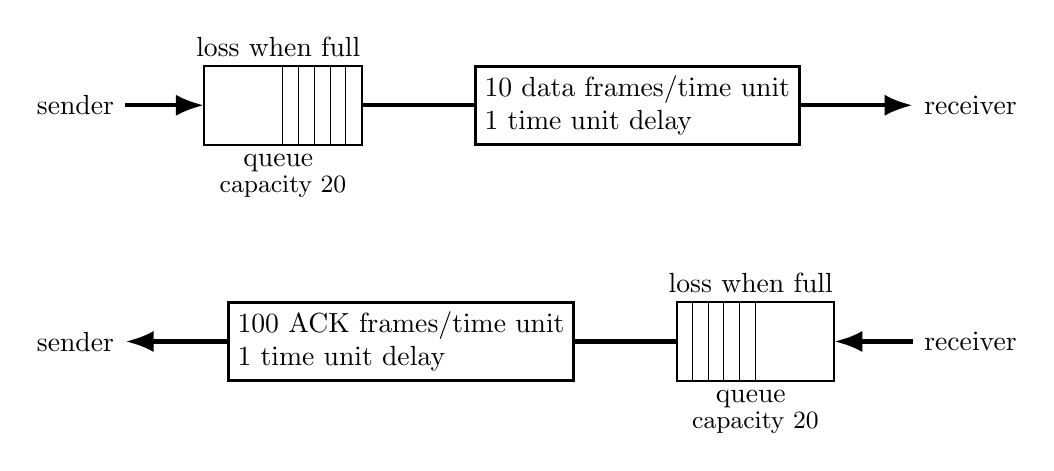
\begin{tikzpicture}
\draw[ultra thick,arrows={-Latex}] (0, 0) node[left] {sender} -- (1, 0);
\draw[thick] (1, -.5) rectangle (3, .5);
\foreach \x in {2,2.2,2.4,2.6,2.8} {
    \draw (\x, -.5) -- (\x, .5);
}
\node[anchor=south,align=center] at (2, .5) {
    loss when full
};
\node[anchor=north,align=center] at (2, -.5) (queue label) {
    queue
};
\node[anchor=north,font=\small] at ([yshift=.2cm]queue label.south) {
    capacity 20
};
\draw[ultra thick,arrows={-Latex}] (3, 0) -- (10, 0) node[right]{receiver}
    node[midway,fill=white,draw=black,very thick,align=left] {
        10 data frames/time unit \\
        1 time unit delay
    };
\begin{scope}[shift={(10, -3)},x=-1cm]
    \draw[ultra thick,arrows={-Latex}] (0, 0) node[right] {receiver} -- (1, 0);
    \draw[thick] (1, -.5) rectangle (3, .5);
    \foreach \x in {2,2.2,2.4,2.6,2.8} {
        \draw (\x, -.5) -- (\x, .5);
    }
    \node[anchor=south,align=center] at (2, .5) {
        loss when full
    };
    \node[anchor=north,align=center] at (2, -.5) (queue label) {
        queue
    };
    \node[anchor=north,font=\small] at ([yshift=.2cm]queue label.south) {
        capacity 20
    };
    \draw[ultra thick,arrows={-Latex}] (3, 0) -- (10, 0) node[left]{sender}
        node[midway,fill=white,draw=black,very thick,align=left] {
            100 ACK frames/time unit \\
            1 time unit delay
        };
\end{scope}
\end{tikzpicture}
\begin{itemize}
\item simulator from upcoming assignment
    \begin{itemize}
    \item command line \texttt{--delay 1 --bandwidth-forward 10 --bandwidth-backward 100 --buffer 30}
    \end{itemize}
\end{itemize}
\end{frame}

\begin{frame}{exercise: forward latency}
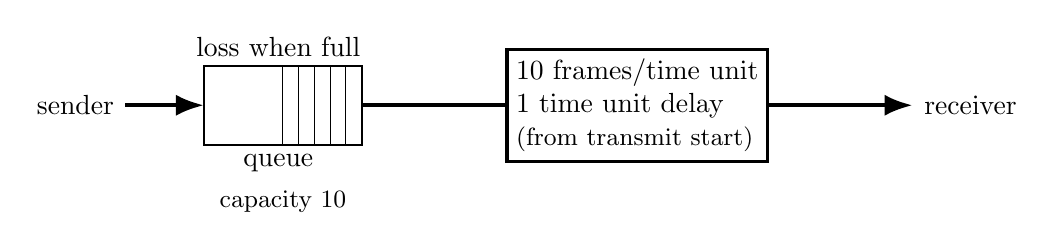
\begin{tikzpicture}
\draw[ultra thick,arrows={-Latex}] (0, 0) node[left] {sender} -- (1, 0);
\draw[thick] (1, -.5) rectangle (3, .5);
\foreach \x in {2,2.2,2.4,2.6,2.8} {
    \draw (\x, -.5) -- (\x, .5);
}
\node[anchor=south,align=center] at (2, .5) {
    loss when full
};
\node[anchor=north,align=center] at (2, -.5) (queue label) {
    queue
};
\node[anchor=north,font=\small] at (queue label.south) {
    capacity 10
};
\draw[ultra thick,arrows={-Latex}] (3, 0) -- (10, 0) node[right]{receiver}
    node[midway,fill=white,draw=black,very thick,align=left] {
        10 frames/time unit \\
        1 time unit delay \\
        \small (from transmit start)
    };
\end{tikzpicture}
\begin{itemize}
\item minimum latency = 1 time unit
\item exercise: maximum latency?
\end{itemize}
\begin{tabular}{lll}
A. 1 time unit & B. 1.1 time unit & C. 1.2 time unit \\
C. 1.4 time unit & D. 1.9 time unit & E. 2.0 time unit \\
F. 2.1 time unit & G. something else \\
\end{tabular}
\end{frame}

\begin{frame}{throughput and window size}
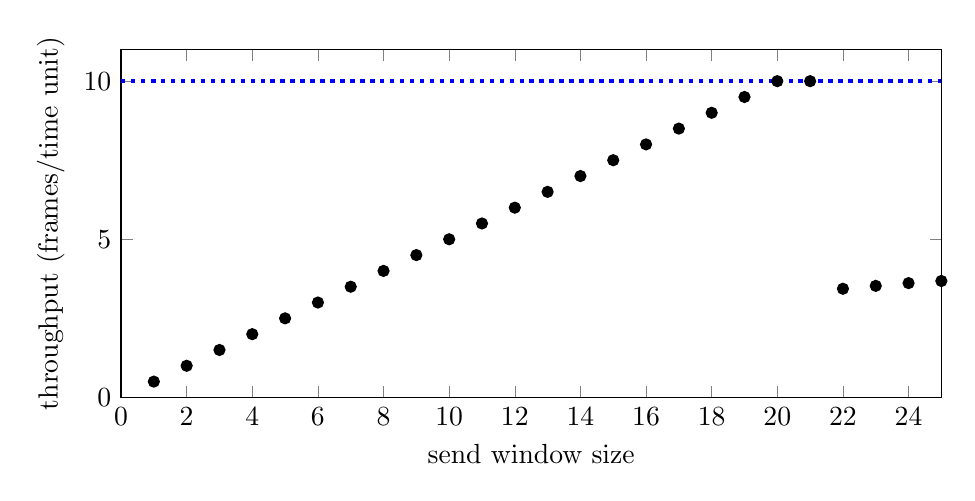
\begin{tikzpicture}
\begin{axis}[width=12cm,height=6cm,
    xlabel=send window size,
    ylabel=throughput (frames/time unit),
    xmin=0,xmax=25,ymin=0]
\addplot[only marks] coordinates {
(1, 0.5000025000125)
(2, 1.0000090000810007)
(3, 1.4999925000374998)
(4, 2.0000280003920055)
(5, 2.500037500562508)
(6, 3.000003000003)
(7, 3.5000035000035)
(8, 4.000048000576006)
(9, 4.499842505512307)
(10, 5.000025000125)
(11, 5.499975250111374)
(12, 5.99977200866367)
(13, 6.499710762871052)
(14, 6.999811005102861)
(15, 7.4996812635462975)
(16, 7.999680012799485)
(17, 8.499426288725509)
(18, 8.999361045365776)
(19, 9.499202067026369)
(20, 9.999100080971061)
(21, 9.999100080973866)
(22, 3.435635094325549)
(23, 3.5274986154570636)
(24, 3.613708966335035)
(25, 3.6808686850100703)
(26, 3.753260645186032)
(27, 3.8487443471573166)
(28, 3.925956461143474)
};
\addplot[blue,dotted,ultra thick,domain=0:25] {10};
\end{axis}
\end{tikzpicture}
\end{frame}

\begin{frame}[fragile,label=transitTime]{packet transit time}
\begin{tikzpicture}
\draw[ultra thick,arrows={-Latex}] (0, 0) node[left] {sender} -- (1, 0);
\draw[thick] (1, -.5) rectangle (3, .5);
\foreach \x in {2,2.2,2.4,2.6,2.8} {
    \draw (\x, -.5) -- (\x, .5);
}
\node[anchor=south,align=center] at (2, .5) {
    loss when full
};
\node[anchor=north,align=center] at (2, -.5) (queue label) {
    queue
};
\node[anchor=north,font=\fontsize{9}{10}\selectfont] at ([yshift=.3cm]queue label.south) {
    capacity 20
};
\draw[ultra thick,arrows={-Latex}] (3, 0) -- (12, 0) node[right]{receiver}
    node[midway,fill=white,draw=black,very thick,align=left] {
        10 data frames/time unit \\
        1 time unit delay
    }
    node[visible on=<1-3>,ultra thick,pos=0,draw=black,fill=white,font=\tiny,below=.5cm] (data-main) {data};
    \begin{visibleenv}<2->
    \draw[red,-Latex,very thick] (data-main.east) -- (data-main.west -| 13, 0) coordinate (end send)
        node[midway,below,font=\small] {1 time unit (sender to receiver)};
    \end{visibleenv}
\begin{scope}[shift={(12, -4)},x=-1cm]
    \draw[ultra thick,arrows={-Latex}] (0, 0) node[right] {receiver} -- (1, 0);
    \draw[thick] (1, -.5) rectangle (3, .5);
    \foreach \x in {2,2.2,2.4,2.6,2.8} {
        \draw (\x, -.5) -- (\x, .5);
    }
    \node[anchor=south,align=center] at (2, .5) {
        loss when full
    };
    \node[anchor=north,align=center] at (2, -.5) (queue label) {
        queue
    };
    \node[anchor=north,font=\small] at ([yshift=.2cm]queue label.south) {
        capacity 20
    };
    \draw[ultra thick,arrows={-Latex}] (3, 0) -- (12, 0) node[left]{sender}
        node[midway,fill=white,draw=black,very thick,align=left] {
            100 ACK frames/time unit \\
            1 time unit delay
        }
        node[visible on=<2->,pos=0,draw=red,fill=white,font=\tiny,below=.5cm,align=center,inner sep=0.5mm] 
            (ack-start) {a\\c\\k};
    \begin{visibleenv}<2->
        \draw[dotted,red,-Latex,very thick] (end send) |- (ack-start.east);
        \draw[red,-Latex,very thick] (ack-start.west) -- (ack-start.west -| 12, 0) node[midway,below,font=\small] { + 1 time unit (receiver to sender)};
    \end{visibleenv}
\end{scope}
\begin{visibleenv}<3>
\node[draw=red,fill=white,ultra thick,align=left] at (6, -2.5) {
    takes 1 + 1 time units to send message + receive ack \\
    goal: keep sending stuff while waiting
};
\end{visibleenv}
\end{tikzpicture}
\end{frame}

\begin{frame}{filling the pipe}
    \begin{itemize}
    \item round-trip time of 2 time units
        \begin{itemize}
        \item from send data to receive ACK (assuming no queuing delay)
        \end{itemize}
    \item can send 10 data frames per time unit
    \item = can send 20 data frames while waiting for ACK
    \end{itemize}
\end{frame}

\begin{frame}[fragile,label=fullPipe]{filling the pipe}
\begin{tikzpicture}
\draw[ultra thick,arrows={-Latex}] (0, 0) node[left] {sender} -- (1, 0);
\draw[thick] (1, -.5) rectangle (3, .5);
\foreach \x in {2,2.2,2.4,2.6,2.8} {
    \draw (\x, -.5) -- (\x, .5);
}
\node[anchor=south,align=center] at (2, .5) {
    loss when full
};
\node[anchor=north,align=center] at (2, -.5) (queue label) {
    queue
};
\node[anchor=north,font=\fontsize{9}{10}\selectfont] at ([yshift=.3cm]queue label.south) {
    capacity 20
};
\draw[ultra thick,arrows={-Latex}] (3, 0) -- (12, 0) node[right]{receiver}
    node[midway,fill=white,draw=black,very thick,align=left] {
        10 data frames/time unit \\
        1 time unit delay
    }
    \foreach \x in {0,1,2,3,4,5,6,7,8,9} {
        node[visible on=<3->,pos=\x*.1+0.05,draw=black,fill=white,font=\tiny,below=.5cm] (data-\x) {data}
    };
    \begin{visibleenv}<3->
    \draw[red,Latex-Latex] ([yshift=-.1cm]data-0.south west) -- ([yshift=-.1cm]data-1.south west)
        node[below,font=\small] {0.1 time unit};
    \end{visibleenv}
\begin{scope}[shift={(12, -4)},x=-1cm]
    \draw[ultra thick,arrows={-Latex}] (0, 0) node[right] {receiver} -- (1, 0);
    \draw[thick] (1, -.5) rectangle (3, .5);
    \foreach \x in {2,2.2,2.4,2.6,2.8} {
        \draw (\x, -.5) -- (\x, .5);
    }
    \node[anchor=south,align=center] at (2, .5) {
        loss when full
    };
    \node[anchor=north,align=center] at (2, -.5) (queue label) {
        queue
    };
    \node[anchor=north,font=\small] at ([yshift=.2cm]queue label.south) {
        capacity 20
    };
    \draw[ultra thick,arrows={-Latex}] (3, 0) -- (12, 0) node[left]{sender}
        node[midway,fill=white,draw=black,very thick,align=left] {
            100 ACK frames/time unit \\
            1 time unit delay
        }
        \foreach \x in {0,1,2,3,4,5,6,7,8,9} {
            node[visible on=<3->,pos=\x*.1+0.05,draw=black,fill=white,font=\tiny,below=.5cm,align=center,inner sep=0.5mm] {a\\c\\k}
        };
\end{scope}
\end{tikzpicture}
\end{frame}
